\section{结果}

\subsection{通用基准与历史 SeNPs 分组预测}

通用数据的固定预算文献分组评价得到 RF 的 OOF MAE 为 21.71 个百分点、RMSE 为 28.46 个百分点、$R^2=0.150$，XGBoost 分别为 22.54 个百分点、29.72 个百分点和 0.073。该结果提供了当前通用输入与分组条件下的基准，不能与旧稿中随机划分的深度模型或分类指标合并为一次统一模型排名。

历史 SeNPs 的严格主分析中，基础 RF 的 OOF MAE 为 19.11 个百分点，XGBoost 为 19.49 个百分点，两者的 $R^2$ 均较低（表~\ref{tab:senp_main_results}）。化学增强没有降低按样本汇总的 MAE，RF 相对基础配置增加 0.180 个百分点，XGBoost 增加 0.030 个百分点；RF 的文献组等权差值为 +0.183，bootstrap 95\% 区间为 $[0.054,0.333]$，XGBoost 对应区间跨越 0。当前可用化学字段没有表现出稳定的预测收益，RF 的组等权结果还显示小幅误差增加。

\begin{table}[htbp]
\centering
\caption{434 条历史 SeNPs 记录的 5 折外层、3 折内层文献分组评价。指标由外层 OOF 预测计算，IC50 辅助配置单列。}
\label{tab:senp_main_results}
\small
\begin{tabular}{llrrr}
\toprule
模型 & 特征配置 & MAE（百分点） & RMSE（百分点） & R\textsuperscript{2} \\
\midrule
RF & 基础 & 19.11 & 24.12 & 0.109 \\
XGBoost & 基础 & 19.49 & 23.97 & 0.120 \\
RF & 化学增强，不含 IC50 & 19.29 & 24.25 & 0.099 \\
XGBoost & 化学增强，不含 IC50 & 19.52 & 23.87 & 0.128 \\
RF & IC50 辅助 & 18.97 & 24.13 & 0.109 \\
XGBoost & IC50 辅助 & 18.35 & 23.25 & 0.172 \\
\bottomrule
\end{tabular}

\end{table}

IC50 辅助 XGBoost 的 MAE 数值最低，但该输入来自毒性响应，使用前提与基础模型不同。它相对基础模型的样本等权 MAE 降低 1.145 个百分点，文献组等权差值为 $-0.835$，95\% 区间为 $[-3.296,1.531]$，未显示稳定改善。所有配对比较的两个估计量与对应区间见补充表~\ref{tab:paired_comparisons}，不以最小单个误差值替代主模型的使用条件。

\subsection{迁移与剂量—时间交互的预测增量}

固定 500 树预算下，General zero-shot 在 SeNPs 上的误差高于 SeNP-only，迁移也没有形成稳定收益（表~\ref{tab:transfer_results}）。RF 迁移的样本等权 MAE 增加 0.577 个百分点，XGBoost 降低 0.669 个百分点，但对应的文献组等权差值区间分别为 $[-2.763,1.414]$ 与 $[-1.417,1.317]$，均跨越 0。这些结果限定于当前共同特征与树模型迁移方式，尚不足以认为通用数据能直接改善 SeNPs 的跨文献预测。

\begin{table}[htbp]
\centering
\caption{固定 500 树预算的 General 到 SeNP 迁移对照。该对照采用预先指定参数，与表~\ref{tab:senp_main_results} 的嵌套选择主分析分别解释。}
\label{tab:transfer_results}
\small
\begin{tabular}{llrrr}
\toprule
模型 & 策略 & MAE（百分点） & RMSE（百分点） & $R^2$ \\
\midrule
RF & SeNP-only & 19.72 & 24.98 & 0.045 \\
RF & General zero-shot & 23.72 & 30.96 & -0.467 \\
RF & General→SeNP & 20.30 & 25.77 & -0.017 \\
XGBoost & SeNP-only & 20.75 & 26.09 & -0.042 \\
XGBoost & General zero-shot & 23.44 & 29.54 & -0.336 \\
XGBoost & General→SeNP & 20.08 & 25.49 & 0.006 \\
\bottomrule
\end{tabular}

\end{table}

加入显式剂量—时间交互后，RF 与 XGBoost 的样本等权 MAE 分别增加 0.392 和 0.605 个百分点，文献组等权区间均跨越 0（补充表~\ref{tab:paired_comparisons}）。显式交互项未提供稳定预测增量，该结果不排除真实实验中存在时间相关响应，也不等同于模型已准确学习新增实验的二维响应。

\subsection{HUVEC 中的剂量—时间观测与材料差异}

新增工作簿完整覆盖 9 种材料、3 个时间点和 13 个浓度水平，没有缺失字段或重复条件键，共形成 27 条曲线。存活率报告范围为 6.13\%—121.61\%，其中 60 个报告值高于 100\%，全部曲线都存在相邻浓度间的局部上升，因此保留原始报告点而不强制单调拟合（图~\ref{fig:huvec_dose_time}）。归档表中的零浓度报告值均为 100\%，其原始归一化与空白扣除流程仍需依据实验记录核实。

\begin{figure}[htbp]
\centering
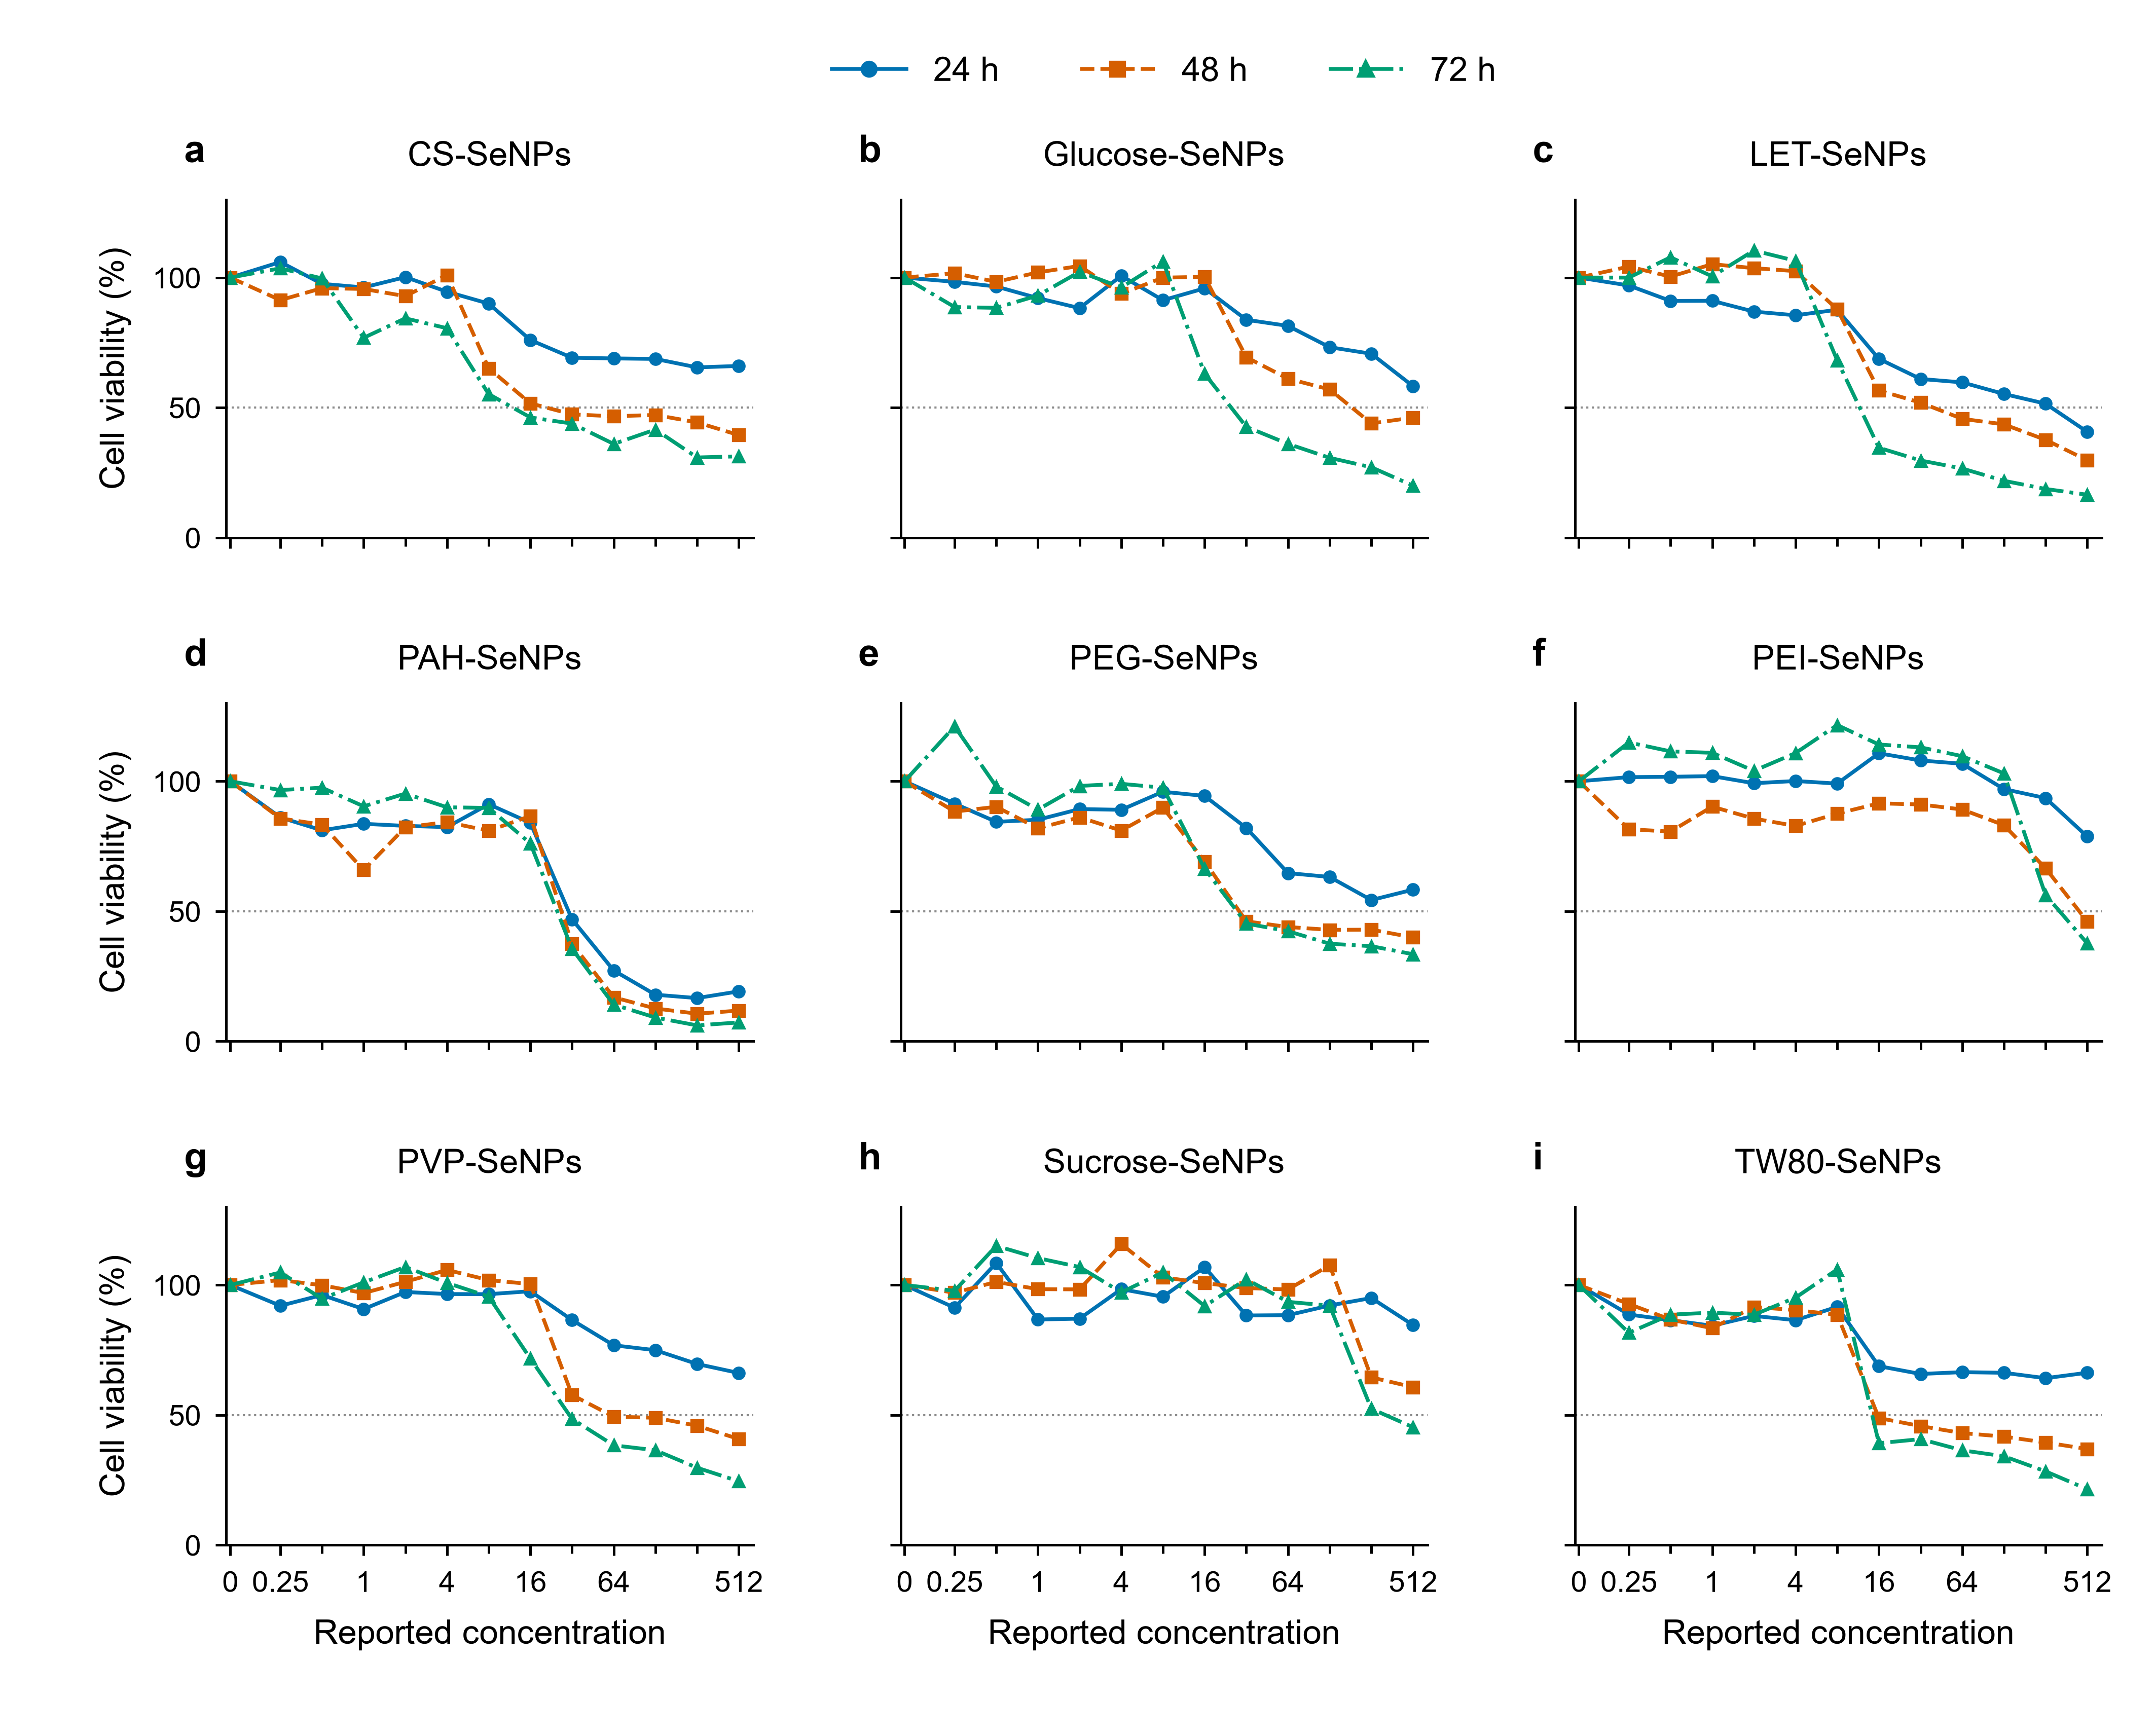
\includegraphics[width=\linewidth]{figures/huvec-dose-time.png}
\caption{9 种 SeNPs 在 HUVEC 中的剂量—时间报告曲线。a—i 依次为 CS、Glucose、LET、PAH、PEG、PEI、PVP、Sucrose 与 TW80，颜色、点形和线型区分 24、48、72 h。每条曲线包含 13 个报告点，横轴正浓度区采用以 2 为底的对数尺度，零点附近采用线性段以保留对照，浓度单位的含义与计量基准待核实。连线只连接报告点，灰色虚线表示 50\% 存活率；每个条件的重复次数与汇总方法未提供，图中不绘制误差条。}
\label{fig:huvec_dose_time}
\end{figure}

最高报告浓度 512 下，9 种材料的平均存活率在 24、48、72 h 分别为 59.81\%、39.07\% 和 26.38\%，24 h 至 72 h 下降 33.42 个百分点，九种材料在该浓度下均随时间延长而降低。该结果表明当前 HUVEC 观测具有高浓度下的时间依赖性，平均值描述的是不同材料的等权汇总，不是重复孔均值或实验误差估计。

在 HUVEC、72 h、报告浓度 512 下，PAH-SeNPs 的存活率最低，为 7.26\%，Sucrose-SeNPs 最高，为 45.30\%（表~\ref{tab:huvec_materials}）。其余材料按存活率递增依次为 LET、Glucose、TW80、PVP、CS、PEG 和 PEI，这一排序只描述指定条件下的观测差异，不代表所有剂量与时间下的统一安全性排序。

\begin{table}[htbp]
\centering
\caption{报告浓度 512 下的材料描述符与 HUVEC 存活率。按 72 h 存活率递增排列，每种材料的粒径和 Zeta 电位均为工作簿提供的固定报告值。}
\label{tab:huvec_materials}
\small
\begin{tabular}{lrrrrr}
\toprule
材料 & 粒径（nm） & Zeta（mV） & 24 h（\%） & 48 h（\%） & 72 h（\%） \\
\midrule
PAH-SeNPs & 190.72 & 51.70 & 19.21 & 11.82 & 7.26 \\
LET-SeNPs & 107.56 & \ensuremath{\mathord{-}}27.52 & 40.67 & 29.73 & 16.49 \\
Glucose-SeNPs & 115.82 & \ensuremath{\mathord{-}}23.83 & 58.25 & 46.16 & 19.98 \\
TW80-SeNPs & 78.03 & \ensuremath{\mathord{-}}21.90 & 66.26 & 36.93 & 21.48 \\
PVP-SeNPs & 143.76 & \ensuremath{\mathord{-}}31.79 & 66.16 & 40.78 & 24.52 \\
CS-SeNPs & 114.72 & 33.36 & 66.02 & 39.44 & 31.25 \\
PEG-SeNPs & 111.96 & \ensuremath{\mathord{-}}37.07 & 58.32 & 39.96 & 33.49 \\
PEI-SeNPs & 214.58 & 24.77 & 78.74 & 46.10 & 37.67 \\
Sucrose-SeNPs & 184.60 & 12.97 & 84.61 & 60.72 & 45.30 \\
\bottomrule
\end{tabular}

\end{table}

\subsection{表观 IC50 与描述符的探索性关联}

27 条曲线中，19 条存在唯一的相邻正浓度 50\% 括区，可得到表观 \IC，另外 8 条在测试范围内始终高于 50\%，记为 $>512$。可插值曲线在 24、48、72 h 分别为 2、8、9 条，有限估计在原始浓度尺度上为 11.63—448.56；完整结果见补充表~\ref{tab:huvec_ic50}，相邻点和状态保留在源数据表中。

表观 \IC 与最高浓度下的存活率描述不同的曲线特征，两者的材料排序并不完全一致。72 h 时，LET-SeNPs 的表观 \IC 最低，为 11.63，PAH-SeNPs 为 25.00，但 PAH-SeNPs 在报告浓度 512 下的存活率更低。对材料进行比较需要先明确评价时间、浓度范围和采用的曲线指标，不能将一个高浓度点的排序直接推广为全部剂量区间的排序。

在报告浓度 512 下，以 9 种材料为分析单位，粒径与 24、48、72 h 存活率的 Spearman 系数分别为 0.200、0.383 和 0.267，Zeta 电位对应值为 0.050、$-0.183$ 和 $-0.050$。这些描述性系数没有形成稳定的单变量关联证据，当前记录也不能区分粒径、电位、修饰化学及其他未测量因素的独立作用。新增实验尚未与事先封存的模型预测配对，因此这里不报告新材料预测的 MAE、RMSE、$R^2$、预测—实测排序相关或预测 \IC 误差。
\FloatBarrier
